\section{Target Group}
\begin{figure}[H]
\centering
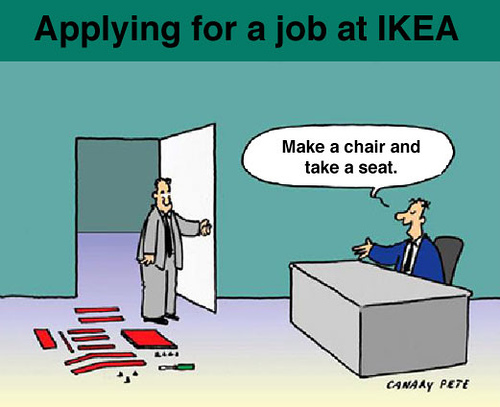
\includegraphics[scale=0.5]{IKEAInterview.jpg}
%\caption{iPhone game using a gyroscope sensor}
\end{figure}
Profound understanding of the target group helps to create useful concept - it will be answer to users specific needs and wishes. Dividing target group to different group categorizations - segments, gives possibility to understand chosen subject deeper and hopefully it leads to better project. Prototype design will be specifically designed for segmented and generalized group of people of this project. Connecting with target group is essential since product will be used by actual customers. It is not enough to generalize group of people from surface observations or believed stereotypes, since sometimes people do not act as they speak and actual needs can vary a lot. In target group section, detailed information about users of IKEA will be revealed.

This project is targeting at people who are IKEA shop’s customers and who are newly decorating or changing furniture, decor of their home. This part of research includes two parts - understanding people who has need for application that we develop, and IKEA’s target group - people that Ikea attracts  and who are coming to shop for furniture or decor.

There are many ways to segment target audience. Probably most popular is Geographic or Demographic segmentation. In this case we will go deeper and have a look at Psychographics too - we want to know specific needs of customers which will help to design helpful app. 

\subsection{Demographics }
Demographics is segmenting that describes group of people according age, gender, family size and life cycle (examstutor.com, Demographics). This segment gives core for understanding the audience and it helps to start creating other generalizations as psychographics.

\subsubsection{What is IKEA targeted customer's age ?}
Checking IKEA’s report, public documentations, websites -  it is not clear to see what range of age people IKEA is trying to attract. Contacting IKEA also did not result in finding out their specific target group’s age range. According observations and descriptions of center, IKEA’s targeted group age range is really wide - there are lounges for children, considerations for disabled and old people. At “IKEA’S Accessibility Plan” (Accessibility Plan, 2013) they mention that there are consideration to accept people from children to old aged or disabled people. Report even states that staff is trained to help people with disabilities, their equipment and even help-animals. All IKEA shops has mini restaurants where different range of age people can eat. They serve special menus for children, sell wine, and has quick walk-by coffee machines. Assumption can be made that IKEA is trying to appeal to all age range and has not created clear concept design around specific life-cycle stage (examstutor.com, Demographics) nor age range. 
However, according to two interview sessions that were done in local IKEA center of Copenhagen, it was more clear who is shopping there. Majority of interviewed people were young people - between 25 and 35 years of age.

\subsubsection{gender}
IKEA clearly does not mention anything about attracting either men or women to shop in public documentation (Accessibility Plan 2013) nor in their website of Ikea.dk. This was also clear to see through observation in IKEA. However it was interesting to see that at least half of people were shopping together: in couples, friends or family. 
\subsubsection{Social-class}
Age and statistical information of Denmark can reveal which life cycle customers of IKEA could belong to. Picture below shows  “Life-cycle” stages.
\begin{figure}[H]
\centering
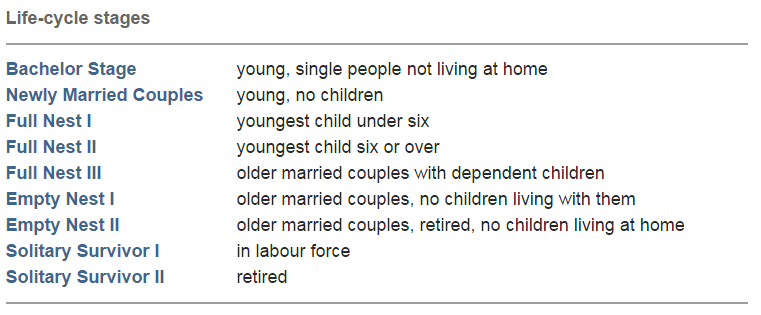
\includegraphics[scale=1]{life_cycle.png}
\caption{Picture from internet -  examtutors.com - demographics}
\end{figure}
Targets group’s maximum age was set to 35, according “Statistics denmark” section “The average dane” woman gives first birth at age of 29.(Statistics Denmark 2014 - The Average Dane) This means that targeted audience is below “Full nest II” - young families. 
 “Danish Ministry of Education” gathered statistical information of when students begin and end their bachelor (Danish Ministry of Education website - Higher education). In picture below it is seen at which age danish students start higher education.
\begin{figure}[H]
\centering
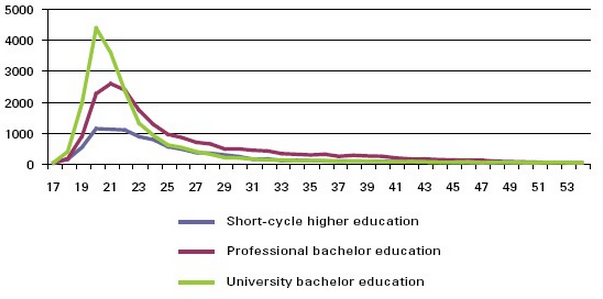
\includegraphics[scale=1]{bachelor.png}
\caption{Picture from internet - Danish Ministry of education - higher education}
\end{figure}
As it is seen in graph above, students finishing bachelor at around age of 25. It means that IKEA attracts people who are just finished some higher education and\or continuing master and above, since set minimum was 25.

Assumption can be made that IKEA attracts young people - Higher education students, young couples and families and of course exceptions.

\subsection{Psychographics}
Psychographic generalization segments target group according social class, lifestyle and personality characteristics. (Examstutor.com, Psychographics) It is important and relevant to understand customer needs ,their habits and personality since it partially can answer how app concept can be developed. 
Since IKEA is attracting young - up to middle-aged people, it is possible to do more accurate analysis of social class, lifestyle and personality traits of our target group (Examstutor.com,  2015). 
\subsubsection{Economy}
Younger people has less money in general than older generations. As example, statistical graph from US below shows the difference of income.
\begin{figure}[H]
\centering
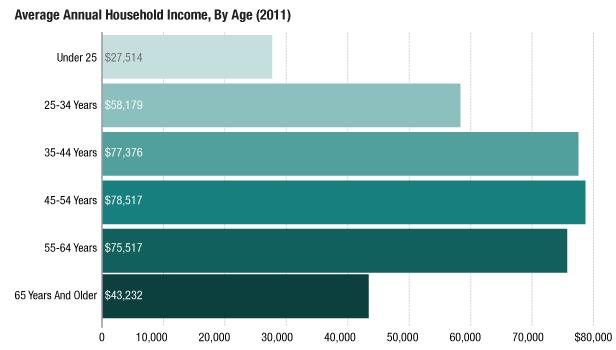
\includegraphics[scale=1]{us_income.jpg}
\caption{Picture from Internet - Income in United States}
\end{figure}

According “examstutor” website, social class is categorized in grade class, where IKEA’s targeted customers could be defined as class C1, C2, D or E:
\begin{figure}[H]
\centering
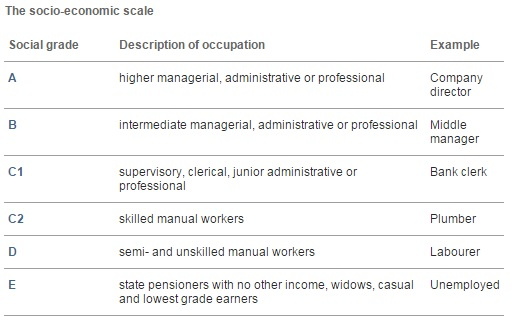
\includegraphics[scale=1]{SocialClassDiagram.jpg}
\caption{Scale of the economic classes}
\end{figure}
People who are lower in socio-economic position in general has less income. IKEA offers low,  furniture prices on market in comparison to other danish-market shops as “Sylvan”, “ILVA” etc - it is easy seen just visiting websites of these shops. Therefore  assumption can be made that younger generation are shopping at IKEA more than other people, because they do care about expenses.  

Interviewing customers confirmed that big half of participants counts their expenses. Furthermore, while interviewing employees of the shop, they noticed that price is one of the most common topic to talk with customers about. This confirms social class categorization mentioned above. 

\subsection{Digital knowledge}
Marc Prensky in his “Digital Natives, Digital Immigrants“ (Prensky, 2001) article categorizes his understanding of target group to two segments,when it comes to understanding or learning with digital technology. He categorizes them to "digital natives" and "digital immigrants".There are few more categorizations that people use as “Born digital” or “Digital Settlers”, so it is common to separate people to “digital knowledge” groups.  Immigrant- is the one who was born and grew up before technology revolution, so for example 65 years old man who did not have all the computers and digital tools or equipment as people do now. This person only adopted to technology at certain age or life point when it was needed. Digital native is the one who grew up in technology era, where he had access for example to Internet, computers, probably experienced one or more ways of learning in digital environment (Prensky, 2001). However, Prensky notes that time will make everyone a "digital native", as everyone will be born in a world full of advanced technology, so old generalization terminology will not be suiting in future. He quotes Albert Einstein - “The problems that exist in the world today cannot be solved by the level of thinking that created them.” Prensky later introduces “Digital wisdom” that is more general but suiting in this era.(M. Prensky, 2008). This “tag” is best suiting to this target group - if IKEA’s customers are young students or people around 35 years of age it means that target group is on the edge of being called both- if person born in 80s or 90s he/she had a chance to learn or use modern technology, depending on geographical and social class of course. That is why terminology of “Digital wisdom” is useful - assumption can be made that most of the target group will be with digital-wisdom. Therefor most of the targeted users should not have huge problems to start using any digital application.

\subsection{Users do plan}
Interviews with target group also gave knowledge that users plan and prepare before going to actual shop. Almost all of interviewed people do some kind of measurements when buying furniture. All interviewed people checks website before going to IKEA, majority do plan before going. 

\subsection{Target group conclusion}
Targeted group of this project are young- middle aged IKEA’s customers from 25 to 35 years of age. Almost every customer has access to personal smartphone and digital-wisdom in using its applications. Targeted people are careful with expenses and considering the price, they also tend to know about the product before actually visiting the shop. Excluding exceptions, IKEA’s customers are graduated or students who study further than bachelor, also young families and couples.



